\documentclass[tikz]{standalone}
\usepackage{tikz}
\usetikzlibrary{automata, positioning}

\begin{document}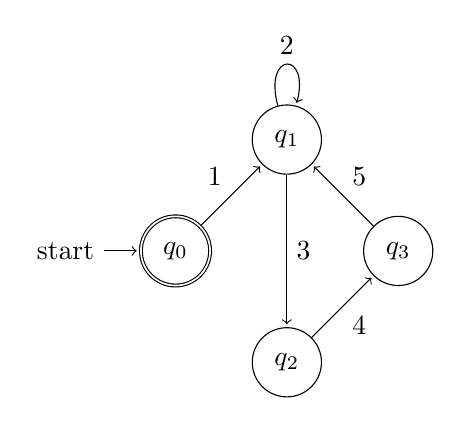
\begin{tikzpicture}[shorten >=1pt, node distance=2cm, on grid, auto]

  \node[state, initial, accepting] (q0) {$q_0$};
  \node[state, above right=of q0] (q1) {$q_1$};
  \node[state, below right=of q0] (q2) {$q_2$};
  \node[state, below right=of q1] (q3) {$q_3$};

  \path[->] (q0) edge node {1} (q1);
  \path[->] (q1) edge [loop above] node {2} (q1);
  \path[->] (q1) edge node {3} (q2);
  \path[->] (q2) edge node [swap] {4} (q3);
  \path[->] (q3) edge node [swap] {5} (q1);

\end{tikzpicture}
\end{document}
